\chapter{Plataforma de desarrollo}
\label{cap:capitulo4}
 
Con los objetivos del proyecto definidos, en este capítulo se abordarán las distintas plataformas de desarrollo, tanto \textit{hardware} como \textit{software}, que han facilitado el logro de esos objetivos.

\section{Hardware}
\label{sec:hardware}

Este apartado recoge la descripción de los componentes \textit{hardware} utilizados en este proyecto, para los cuales se ha buscado priorizar la reducción de costes en cada elección y utilizar aquellos elementos a los que se tenía acceso a la hora del desarrollo del proyecto o de los que se disponía a la hora de elaborarlo.

\subsection{Cámara Logitech C270 HD}
\label{subsec:logiC270HD}

Esta cámara web (Figura \ref{fig:logiC270HD}) de dimensiones 72,91 x 31,91 x 66,64 mm, corrige la iluminación de manera automática, produciendo colores reales y naturales y ajustándose a las condiciones de iluminación del entorno, lo que facilita la detección de fresas. Ofrece una resolución HD 720p, proporcionando imágenes claras y nítidas a una velocidad de 30 fotogramas por segundo (fps) con una lente que cuenta con enfoque fijo y un campo visual diagonal (dFoV) de 55 grados. Su coste aproximado es, en la página oficial, de 44€, aunque en otras empresas destacadas en el sector de la electrónica y la tecnología en España puede encontrarse por, aproximadamente, 25€.

\begin{figure} [H]
    \begin{center}
      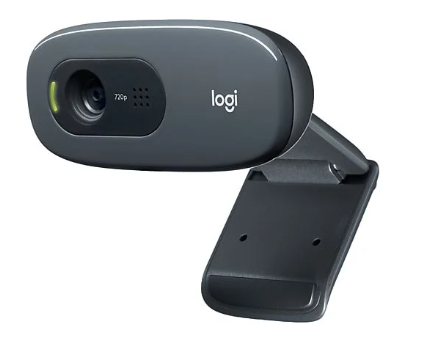
\includegraphics[width=5cm]{figs/logi C270.png}
    \end{center}
    \caption{Cámara Logitech C270 HD$^{\ref{note:enlace16}}$}
    \label{fig:logiC270HD}
\end{figure}

\setcounter{footnote}{16}
\footnotetext[\value{footnote}]{\url{https://www.logitech.com/es-es/products/webcams/c270-hd-webcam.960-001063.html?srsltid=AfmBOor4HptUTcGrxE-4SZxKR-ARw-ykNeagHSEzXUvTlXkx8qLfY4lG}\label{note:enlace16}}

\subsection{Soporte de brazo articulado}
\label{subsec:soporte_camara}

Para poder ubicar la cámara en una posición fija que permitiese visualizar las fresas, se utilizó un soporte de brazo articulado, como el representado en la Figura \ref{fig:soporte_camara}, cuya parte fija en la parte inferior se ancla a la mesa. Este soporte articulado, tiene un ajuste de 360 grados, con su extremo más largo de 75 cm, mientras que la carga máxima que permite es de 560 gramos cuando se coloca de manera horizontal, siendo el precio de este soprte 22,98€.

\begin{figure} [H]
    \begin{center}
      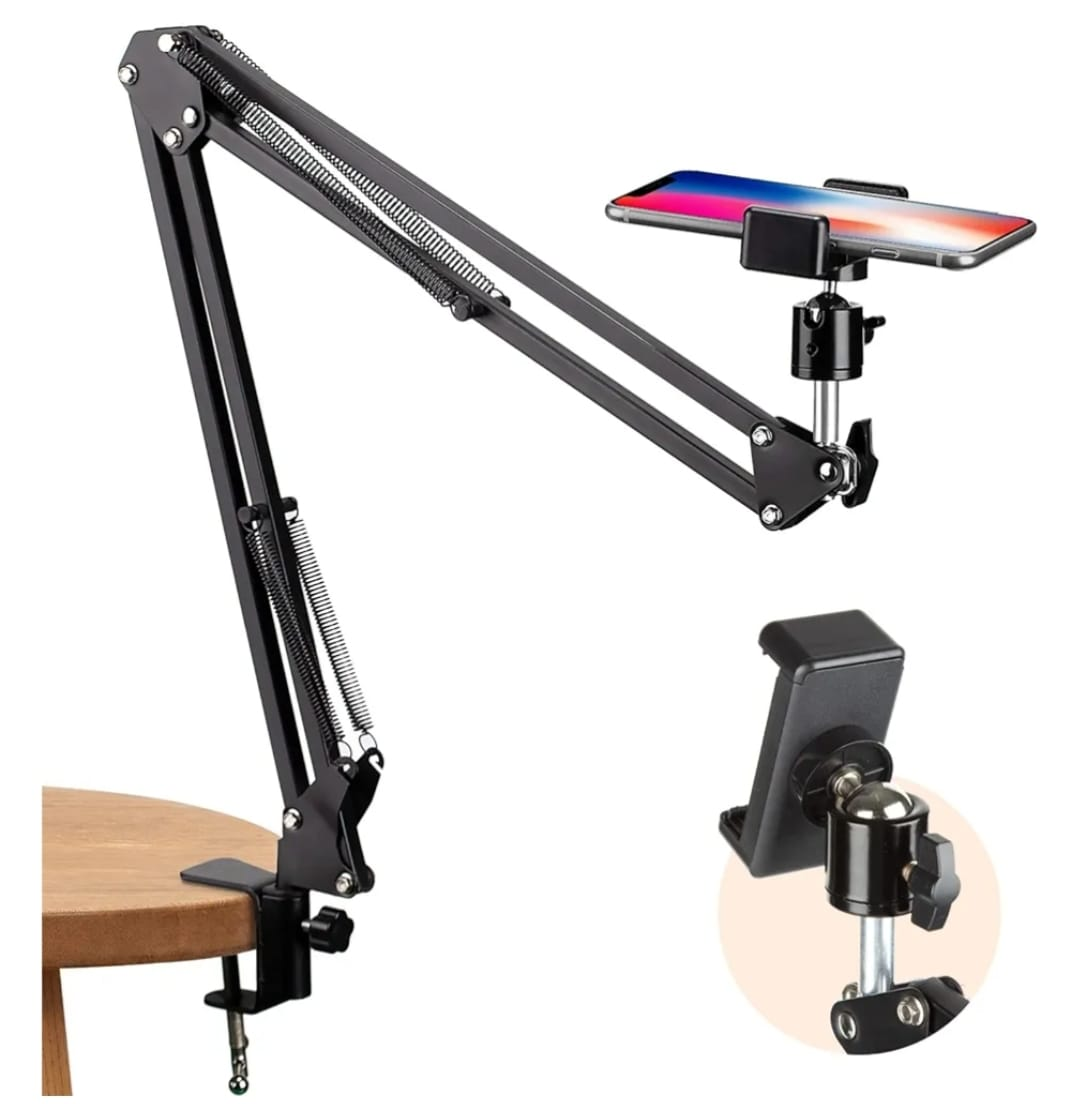
\includegraphics[width=5cm]{figs/Soporte de brazo articulado.jpeg}
    \end{center}
    \caption{Soporte de brazo articulado$^{\ref{note:enlace17}}$}
    \label{fig:soporte_camara}
\end{figure}
 
\setcounter{footnote}{17} 
\footnotetext[\value{footnote}]{\url{https://www.amazon.es/dp/B08JCG4V5S?ref=ppx_pop_mob_ap_share&th=1}\label{note:enlace17}}

\subsection{Ordenador principal}
\label{subsec:ordenador}

El equipo que se ha configurado como entorno de trabajo para este proyecto es el que aparece en la Figura \ref{fig:PC_Lenovo}, sirviendo como base para el desarrollo de la programación y las pruebas de la visión artificial, y utilizándose igualmente como servidor para poder llevar a cabo la comunicación con el brazo robótico mediante el protocolo XML-RPC basado en HTTP, y posteriormente el envío de posiciones detectadas en tiempo real a este. 

\begin{figure} [H]
    \begin{center}
      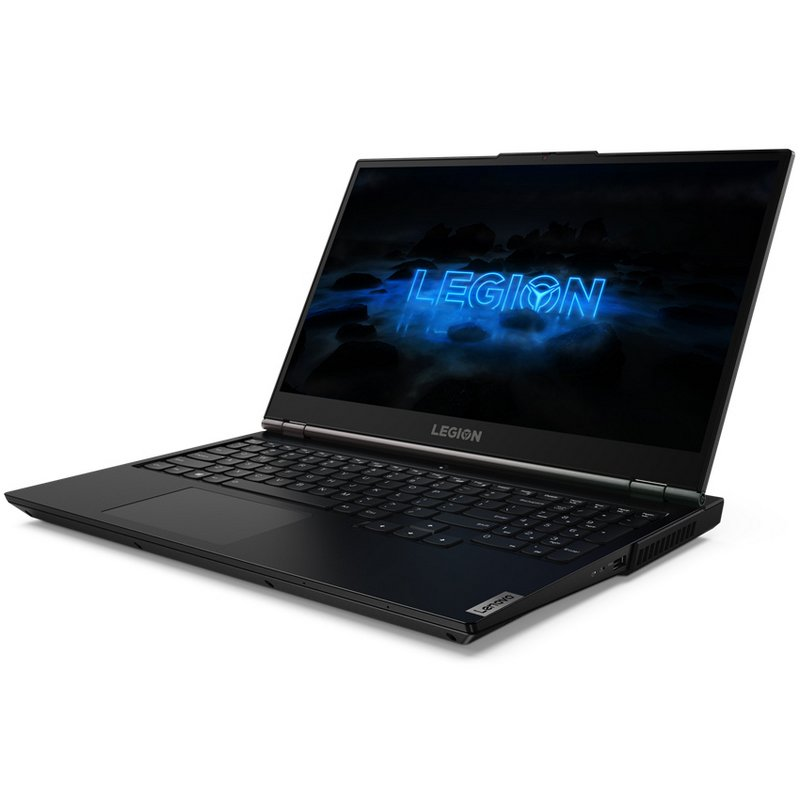
\includegraphics[width=7cm]{figs/Lenovo Legion 5 15imh05.jpg}
    \end{center}
    \caption{Lenovo Legion 5 15IMH05$^{\ref{note:enlace18}}$}
    \label{fig:PC_Lenovo}
\end{figure}

\setcounter{footnote}{18}
\footnotetext[\value{footnote}]{%
    https://www.pccomponentes.com/lenovo-legion-5-15imh05-intel-core-i7-10750h-16gb-1tb-ssd-gtx-1650-156?srsltid=AfmBOopJpvGSHUyQU696jgG7-6orSKMOEWZe2ZvvYtA0NGtJ9Ms2xJFp%
    \label{note:enlace18}%
}
    
A continuación, en el Cuadro \ref{cuadro:carac_ordena}, se recogen las características técnicas del ordenador utilizado:

\begin{table}[H]
	\begin{center}
		\begin{tabular}{|c|c|}
			\hline
			\textbf{Características} & \textbf{Descripción} \\
			\hline
			\multirow{2}{*}{Pantalla} & \multirow{2}{*}{\shortstack{15,6 pulgadas \\ Full HD (1920x1080)}} \\
			& \\
			\hline
			Procesador (CPU) & Intel Core i7-10750H CPU @ 2.60GHz \\
			\hline
			Memoria RAM & 16 GB \\
			\hline
			Almacenamiento & 1 TB \\
			\hline
			Tarjeta gráfica (GPU) & NVIDIA GeForce GTX 1650 Ti Mobile \\
			\hline
			Sistema Operativo & Windows 10 y Ubuntu 22.04.4 LTS \\
			\hline
			Cámara de portátil & HD 720p con tapa de privacidad \\
			\hline
			\multirow{5}{*}{Puertos} & \multirow{5}{*}{\shortstack{4 x USB 3.2 Gen 1 Tipo-A \\ 1 x USB 3.2 Gen 1 Tipo-C \\ 1 x Ethernet (RJ-45) \\ 1 x HDMI 2.0 \\ 1 x combo auriculares/micrófono (3.5 mm)}} \\
			& \\
			& \\
			& \\
			& \\
			\hline
			Conectividad & WiFi 6 802.11ax (2x2), Bluetooth 5.0, Ethernet 100/1000M \\
			\hline
			Batería & 80 Wh \\
			\hline
			Peso & 2,3 kg \\
			\hline
			Dimensiones & 363,06 x 259,61 x 23,57--26,1 mm \\
			\hline
		\end{tabular}
		\caption{Especificaciones técnicas del ordenador usado}
		\label{cuadro:carac_ordena}
	\end{center}
\end{table}

\subsection{Robot de Universal Robots de la gama e-series}
\label{subsec:URe-series}

Los robots de Universal Robots, también conocidos como robots colaborativos o cobots, están diseñados para trabajar junto a los humanos de manera segura, eficiente y flexible tanto en aplicaciones industriales como no industriales, destacando por su facilidad de uso, versatilidad y capacidad para automatizar tareas repetitivas o peligrosas. 

Para el desarrollo de este proyecto se han utilizado diferentes modelos de robots de la gama e-series, todos ellos representados en la Figura \ref{fig:Gama_e-series}, desde el UR3e hasta el UR10e, pasando por el UR5e.
A pesar de que tanto la gama CB-series como la gama e-series permiten la comunicación mediante el protocolo XML-RPC, la interfaz más intuitiva y simplificada que facilita la programación y reduce la sobrecarga de información, poseer sensor de fuerza integrado, permitiendo un control más preciso y sensible haciendo que mejore la interacción con el entorno, así como una mayor precisión en la repetición de movimientos, entre otros factores, constituyeron que se eligiera la gama e-series para este trabajo.

\begin{figure} [H]
    \begin{center}
      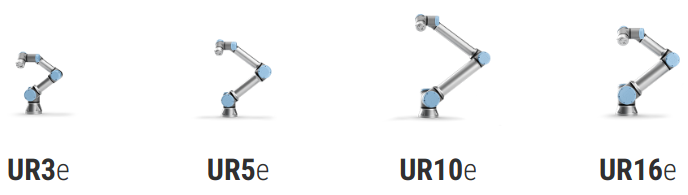
\includegraphics[width=15cm]{figs/Gama e-series.png}
    \end{center}
    \caption{Gama e-series de Universal Robots$^{\ref{note:enlace19}}$}
    \label{fig:Gama_e-series}
\end{figure}

\setcounter{footnote}{19} 
\footnotetext[\value{footnote}]{\url{https://www.universal-robots.com/es/productos/}\label{note:enlace19}}


\section{Software}
\label{sec:software}

Este apartado estará dedicado a detallar las plataformas de software, librerías y entornos de trabajo que han sido fundamentales para alcanzar los objetivos definidos en el Capítulo 3, desde el sistema operativo utilizado hasta las tecnologías específicas para el procesamiento de imágenes y aprendizaje profundo.

\subsection{Ubuntu}
\label{sec:ubuntu}
Ubuntu\footnote{\url{https://ubuntu.com/}} es un sistema operativo de código abierto basado en Linux y desarrollado por la empresa británica Canonical Ltd. 
Este sistema operativo está diseñado para ser utilizado en una gran variedad de dispositivos, y es reconocido por su facilidad de uso, estabilidad y seguridad, contando con una amplia comunidad de desarrolladores y usuarios que contribuyen activamente a su desarrollo y soporte. La versión utilizada para la realización de este proyecto, de entre todas las versiones disponibles, tal y como muestra Figura \ref{fig:Ubuntu_Releases}, es Ubuntu 22.04 Long Term Support (LTS) (Jammy Jellyfish), ya que era la última versión disponible de Ubuntu en el momento en el que se empezó a elaborar el proyecto. Sus principales diferencias con versiones anteriores incluyen el uso de un kernel y versiones de python más modernas, que proporcionan mejor soporte para hardware reciente y optimizaciones de rendimiento, un entorno de escritorio GNOME, que ha evolucionado de Unity en versiones antiguas como 14.04 y 16.04, y  la reducción en el tamaño de las imágenes del sistema, al igual que la optimización del uso de recursos.\\

\begin{figure} [H]
    \begin{center}
      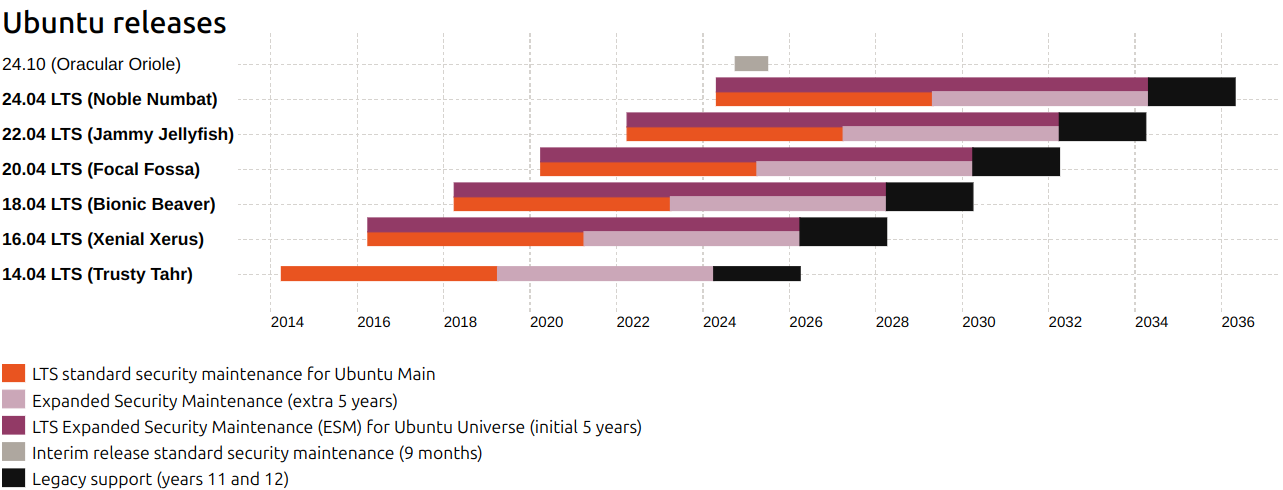
\includegraphics[width=16cm]{figs/Ubuntu Releases.png}
    \end{center}
    \caption{Lanzamiento de las versiones de Ubuntu}
    \label{fig:Ubuntu_Releases}
\end{figure}
\pagebreak


\subsection{Python}
\label{sec:python}
Python\footnote{\url{https://www.python.org/}}(Figura \ref{fig:Python_Logo}) es un lenguaje de programación de alto nivel, orientado a objetos y de semántica dinámica. La sintaxis de Python, sencilla y fácil de aprender, favorece la legibilidad y, por tanto, reduce el coste de mantenimiento de los programas, admitiendo módulos y paquetes, lo que fomenta la modularidad del programa y la reutilización de código \footnote{\url{https://www.python.org/doc/essays/blurb/}} para el desarrollo de aplicaciones en diferentes áreas, como sucede en este caso con la inteligencia y visión artificial y el aprendizaje automático (PyTorch, NumPy y OpenCV). 

\begin{figure} [H]
    \begin{center}
      
\includegraphics[width=10cm]{figs/python logo.png}
    \end{center}
    \caption{Logo de Python}
    \label{fig:Python_Logo}
\end{figure}

\subsection{PyTorch}
\label{sec:PyTorch}

De los desarrolladores de Facebook AI Research junto a otros laboratorios, PyTorch\footnote{\url{https://pytorch.org/}} es un marco de aprendizaje profundo de código abierto conocido por su compatibilidad con Python, siendo un marco de trabajo completo para crear modelos de aprendizaje profundo. Se distingue por su excelente compatibilidad con GPU y su uso de la autodiferenciación en modo inverso, que permite modificar los gráficos de cálculo sobre la marcha, lo que lo convierte en una opción popular para la experimentación rápida y la creación de prototipos.

\subsection{NumPy}
\label{sec:NumPy}

NumPy (Numerical Python)\footnote{\url{https://numpy.org/}} es una biblioteca de Python fundamental para el cálculo numérico, que proporciona un objeto de matriz multidimensional, varios objetos derivados (como matrices y matrices enmascaradas) y un surtido de rutinas para realizar operaciones rápidas con matrices \footnote{\url{https://numpy.org/doc/stable/user/whatisnumpy.html/}}. 

En este proyecto, la biblioteca Numpy se ha utilizado para inicializar matrices y vectores de los parámetros intrínsecos y extrínsecos de la cámara, realizar cálculos geométricos y poder obtener las matrices de rotación y traslación de la cámara, llevar a cabo operaciones matriciales como multiplicaciones e inversiones, y para poder proyectar las coordenadas en el espacio 2D a coordenadas tridimensionales mediante operaciones matriciales, pudiendo obtener posteriormente las distancias a los objetos detectados. 

\subsection{OpenCV}
\label{sec:OpenCV}

OpenCV (Open Source Computer Vision Library)\footnote{\url{https://opencv.org/}} es una biblioteca de software de código abierto diseñada para su uso en aplicaciones de aprendizaje automático y visión artificial. Desarrollado por Intel \footnote{\url{https://www.intel.es}} en 1999, cuenta con más de 2.500 algoritmos optimizados, que incluyen un amplio conjunto de algoritmos de visión por ordenador y aprendizaje automático, que permiten desde el reconocimiento y detección de caras, objetos y acciones humanas en vídeos, hasta el seguimiento de movimientos de estos a tiempo real en vídeo. Además, incluyen herramientas para la creación de modelos y nubes de puntos 3D, la generación de imágenes de alta resolución a partir de múltiples tomas, y la búsqueda de imágenes similares en bases de datos. También ofrecen funcionalidades como la eliminación de ojos rojos, el seguimiento ocular, el reconocimiento de paisajes, y la superposición de realidad aumentada mediante marcadores.

En este proyecto, OpenCV (importado como cv2) se ha usado para poder capturar los frames desde la cámara en tiempo real y mostrarlo en una ventana para poder controlar y verificar que se realizan las detecciones correctamente, para convertir estos frames del formato BGR a RGB, dibujar un rectángulo alrededor de las fresas detectadas, añadiendo la etiqueta de texto correspondiente que indica la clase detectada y la confianza de esta detección; permite detener el bucle principal del programa, terminarlo y salir de este si se presiona la tecla configurada para ello, asegurando que la cámara o el archivo de vídeo no permanezcan bloqueados por el programa y cerrando todas las ventanas de visualización creadas.
\pagebreak

\subsection{XML-RPC}
\label{sec:XMLRPC}

XML-RPC\footnote{\url{https://docs.python.org/es/3.8/library/xmlrpc.html}} es un método de Llamada a Procedimiento Remoto (o RPC en inglés) que usa XML para codificar y tranferir datos entre programas a través de sockets y HTTP como protocolo de transporte. Para muchos lenguajes de programación existen servidores XML-RPC gratuitos, entre otros para: Python, Java, C++ y C.

Debido al uso de Python en el proyecto, se utilizó el paquete \textit{xmlrpc}, que agrupa los módulos tanto de cliente como de servidor que implementan XML-RPC. Con este paquete, el controlador del robot UR puede llamar a métodos/funciones (con parámetros) en un programa/servidor remoto y obtener de vuelta datos estructurados, pudiendo realizar un cálculo complejo mediante su uso, que no está disponible en el lenguaje propio de programación del robot.

\subsection{Anaconda}
\label{sec:Anaconda}

Anaconda\footnote{\url{https://www.anaconda.com/}} es una distribución de código abierto para los lenguajes de programación Python y R, diseñada para facilitar la gestión de paquetes y entornos, así como el despliegue de aplicaciones de ciencia de datos y aprendizaje automático. Ofrece herramientas como conda, un sistema de gestión de paquetes y entornos que funciona en Windows, macOS y Linux; y Anaconda Navigator, una aplicación de escritorio que permite gestionar aplicaciones integradas, paquetes y entornos sin necesidad de utilizar la línea de comandos \footnote{\url{https://docs.anaconda.com/anaconda/}}. 

Para este proyecto se ha hecho uso del programa conda, ya que, utilizando esta herramienta es posible instalar y actualizar paquetes y dependencias y cambiar entre entornos desde el mismo ordneador local, permitiendo que puedan ser mantenidos y ejecutados independientemente sin archivos, directorios y rutas, para que se pueda trabajar con versiones específicas de librerías y/o Python mismo, sin afectar a otros proyectos Python, es decir, no afectando los cambios de un entorno a otros \footnote{\url{https://docs.anaconda.com/reference/glossary/\#conda}}.
\pagebreak

\subsection{YOLOv3}
\label{sec:YOLOv3}

YOLOv3 (You Only Look Once versión 3)\footnote{\url{https://docs.ultralytics.com/es/models/yolov3/}} es un algoritmo de detección de objetos en tiempo real que identifica y localiza múltiples objetos dentro de una imagen o video. Desarrollado por Joseph Redmon y Ali Farhadi en 2018, YOLOv3 es la tercera iteración de la serie YOLO (Figura \ref{fig:YOLO_Logo}), conocida por su capacidad para realizar detecciones rápidas y precisas \cite{Redmon18}. Introdujo el uso de tres escalas diferentes para la detección, aprovechando tres tamaños distintos de núcleos de detección: 13x13, 26x26 y 52x52, lo que mejoró significativamente la precisión de la detección de objetos de diferentes tamaños \footnote{\url{https://docs.ultralytics.com/es/models/yolov3/\#key-features}}. La serie YOLOv3, está diseñada específicamente para tareas de detección de objetos, además, YOLOv3 añadió funciones como predicciones multietiqueta para cada cuadro delimitador y una red extractora de características mejorada. Estos modelos son famosos por su eficacia en diversos escenarios del mundo real, equilibrando precisión y velocidad, lo que los hace adecuados para una amplia gama de aplicaciones \footnote{\url{https://docs.ultralytics.com/es/models/yolov3/\#supported-tasks-and-modes}}.

Esta herramienta ha sido elegida para el entrenamiento del modelo de detección de fresas debido a su eficiencia en el uso de recursos computacionales, lo que lo hace más accesible para sistemas con capacidades limitadas; a la amplia documentación y la comunidad activa existente en torno a YOLOv3, que proporciona recursos valiosos para la implementación y resolución de problemas, lo que es esencial en proyectos académicos con plazos definidos \footnote{\url{https://github.com/ultralytics/yolov3/}}; a la competencia en cuanto a precisión y velocidad de YOLOv3 frente a versiones superiores a pesar de presentar estas ciertas mejoras; y a que YOLOv3 es compatible con entornos de desarrollo ampliamente utilizados en proyectos académicos, como Python y bibliotecas estándar de aprendizaje automático, facilitando su integración en el flujo de trabajo del proyecto.

\begin{figure} [H]
    \begin{center}
      
\includegraphics[width=5cm]{figs/yolo_logo.png}
    \end{center}
    \caption{Logo de YOLO}
    \label{fig:YOLO_Logo}
\end{figure}

\pagebreak
Una vez analizadas las plataformas de software y hardware utilizadas en este trabajo de fin de grado, se procederá a detallar el proceso completo de diseño y desarrollo de la aplicación, lo cual será explicado con detalle en los capítulos siguientes.






